\section{Auswertung}

\subsection{Eckige Stäbe, einseitige Einspannung}

Um den Elastizitätsmodul von den eckigen Stäben bei einseitiger Einspannung zu bestimmen wird zunächst eine Grafik erstellt. Dafür wird die Gesamtauslenkung der eckigen Stäbe bei einseitiger Einspannung D(x) aus den Tabellen \ref{tab:1} und \ref{tab:2} gegen $Lx^2-\frac{x^3}{3}$ aufgetragen. Dabei enstehen die Diagramme in den Abbildungen \ref{fig:bee} und \ref{fig:kee}.

\begin{figure}[H]
    \centering
    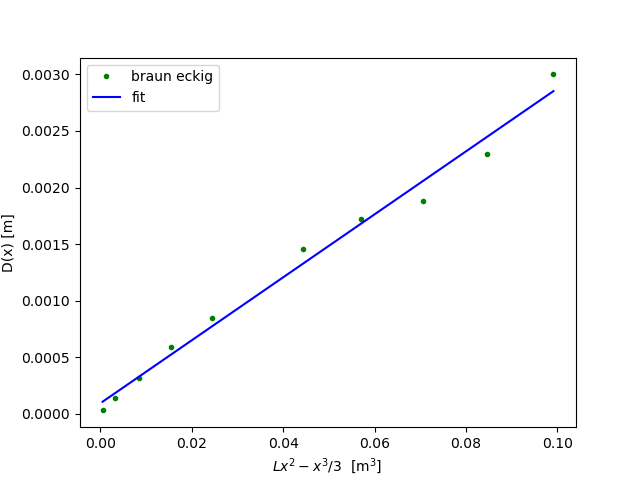
\includegraphics{bee.png}
    \captionof{figure}{Biegung eines braunen, eckigen Stabes mit zugehöriger Ausgleichsrechnung, bei einseitiger Einspannung.}
    \label{fig:bee}
\end{figure}

\begin{figure}[H]
    \centering
    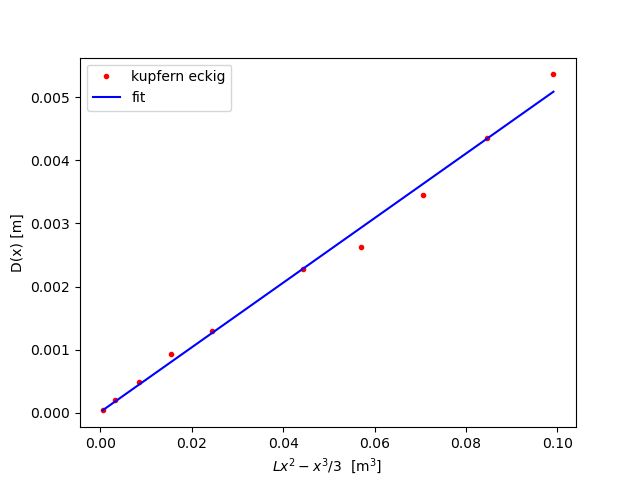
\includegraphics{kee.png}
    \captionof{figure}{Biegung eines kupfernen, eckigen Stabes mit zugehöriger Ausgleichsrechnung, bei einseitiger Einspannung.}
    \label{fig:kee}
\end{figure}

\noindent Die Ausgleichsrechnungen wurden mit der allgemeinen Geradengleichung $y = ax+b$ durchgeführt.
Aus diesen Graphen und den Ausgleichsrechnungen lässt sich der Elastizitätsmodul mit folgender Formel berechnen

\begin{align*}
    E = \frac{m\, g}{2\, I\, a}
\end{align*}

\noindent Dabei ist a die mit der Ausgleichsrechnung bestimmte Steigung der Ausgleichsgeraden. Die Masse m beträgt hier jeweils 1.0543kg.
I ist das Flächenträgheitsmoment. Da die Stäbe Quadratisch sind, ist das Flächenträgheitsmoment $I=\frac{h^4}{12}$.
Beide Stäbe haben als Kantenlänge h=1cm. Die berechneten Parameter sind

\begin{align*}
    a_\text{braun} &= \SI[separate-uncertainty=true]{2.78(0.11)E-2}{\per \square\metre} \\
    b_\text{braun} &= \SI[separate-uncertainty=true]{9.3(5.9)E-5}{\metre} \\
    a_\text{kupfern} &= \SI[separate-uncertainty=true]{5.10(0.16)E-2}{\per \square\metre}\\
    b_\text{kupfern} &= \SI[separate-uncertainty=true]{1.5(8.2)E-5}{\metre}.
\end{align*}

\noindent Diese Abweichungen liefert die von Python durchgeführte Ausgleichsrechnung direkt mit. Mit diesen Werten ergibt sich für die Elastizitätsmodule

\begin{align*}
    E_\text{braun} &=   \SI[separate-uncertainty=true]{223(9)}{\giga\pascal}  \\
    E_\text{kupfern} &= \SI[separate-uncertainty=true]{122(4)}{\giga\pascal}.
\end{align*}

Die Abweichungen der Elastizitätsmodule werden, wegen der Fehlerbehafteten Größe a, mit der Fromel für die Gauß'sche Fehlerfortpflanzung 

\begin{equation} \label{Gauß}
    \Delta y = \frac{\partial y}{\partial x_1} \cdot \Delta x_1 + \frac{\partial y}{\partial x_2} \cdot \Delta x_2 +\cdots \ \Rightarrow \ {u_y}=\sqrt{\left (\frac{\partial y}{\partial x_1} \cdot u_1 \right)^2 +\left (\frac{\partial y}{\partial x_2} \cdot u_2 \right)^2 +\cdots}
\end{equation}

\noindent berechnet.

\subsection{runde Stäbe, einseitige Einspannung}

Für die runden Stäbe ist das Vorgehen identisch zu dem Vorgehen bei den Eckigen. Hier werden die Werte von D(x) aus \ref{tab:3} und \ref{tab:4} genommen. Diese werden genauso gegen $Lx^2-\frac{x^3}{3}$ aufgetragen. Dabei enstehen die Diagramme in den Abbildungen \ref{fig:gre} und \ref{fig:kre}.

\begin{figure}
    \centering
    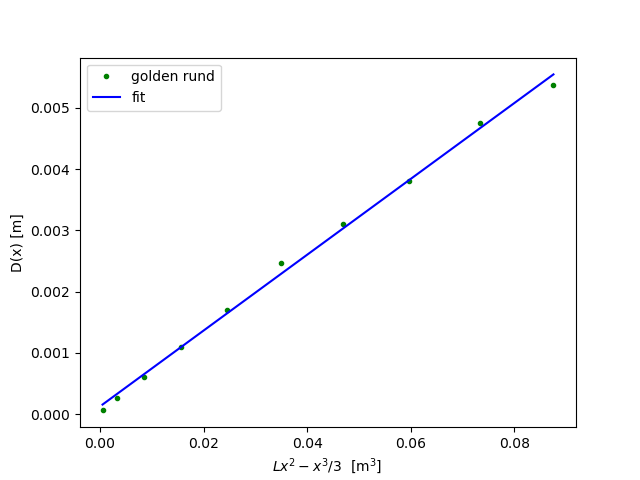
\includegraphics{gre.png}
    \captionof{figure}{Biegung eines goldenen, runden Stabes mit zugehöriger Ausgleichsrechnung, bei einseitiger Einspannung.}
    \label{fig:gre}
\end{figure}

\begin{figure}
    \centering
    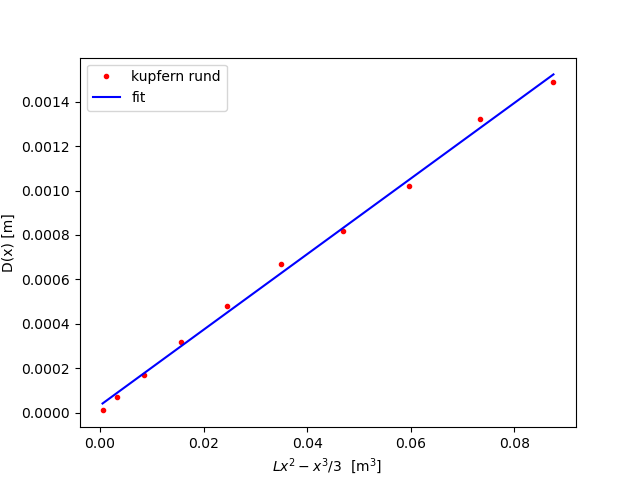
\includegraphics{kre.png}
    \captionof{figure}{Biegung eines kupfernen, runden Stabes mit zugehöriger Ausgleichsrechnung, bei einseitiger Einspannung.}
    \label{fig:kre}
\end{figure}

\noindent Die Ausgleichsrechnung liefert hier folgende Werte

\begin{align*}
    a_\text{golden} &= \SI[separate-uncertainty=true]{6.19(0.12)E-2}{\per \square\metre} \\
    b_\text{golden} &= \SI[separate-uncertainty=true]{1.26(0.53)E-4}{\metre} \\
    a_\text{kupfern} &= \SI[separate-uncertainty=true]{1.70(0.03)E-2}{\per \square\metre}\\
    b_\text{kupfern} &= \SI[separate-uncertainty=true]{3.3(1.6)E-5}{\metre}.
\end{align*}

\noindent Auch die Formel für den Elastizitätsmodul und dessen Fehler (Gleichung \ref{Gauß}) bleiben gleich. Die einzigen Unterschiede sind hier das Flächenträgheitsmoment und die an den Stab gehängte Masse. Die Masse beträgt 0.2492kg für den kupfernen Stab und 0.552kg für den Messingstab. Das Flächenträgheitsmoment lässt sich aufgrund des runden Querschnitts nun folgendermaßen bestimmen

\begin{align*}
    I=\frac{\pi R^4}{4}.
\end{align*}

\noindent Der Durchmesser der beiden Stäbe beträgt 1cm.

\noindent Nun lassen sich wieder die Elastizitätsmodule bestimmen

\begin{align*}
    E_\text{kupfern} &= \SI[separate-uncertainty=true]{146.5(2.6)}{\giga\pascal} \\
    E_\text{golden} &=  \SI[separate-uncertainty=true]{89(17)}{\giga\pascal}.
\end{align*}

\subsection{eckige Stäbe, beidseitige Einspannung}

Für die eckigen Stäbe bei beidseitiger Einspannung werden Werte für D(x) aus den Tabellen \ref{tab:1} und \ref{tab:2} in Diagrammen aufgetragen. Dabei werden jeweils die Werte links vom Aufhängungspunkt (27.5cm) und rechts vom Aufhängungspunkt gesondert aufgetragen. Die Werte links vom Aufhängungspunkt werden dabei gegen $3L^2x-4x^3$ und die Werte rechts vom Aufhängungspunkt gegen $4x^3-12Lx^2+9L^2x-L^3$ aufgetragen. Anschließend wird bei allen Graphen eine lineare Ausgleichsrechnung durchgeführt. Dabei entstehen folgende Diagramme:

\begin{figure}[H]
    \centering
    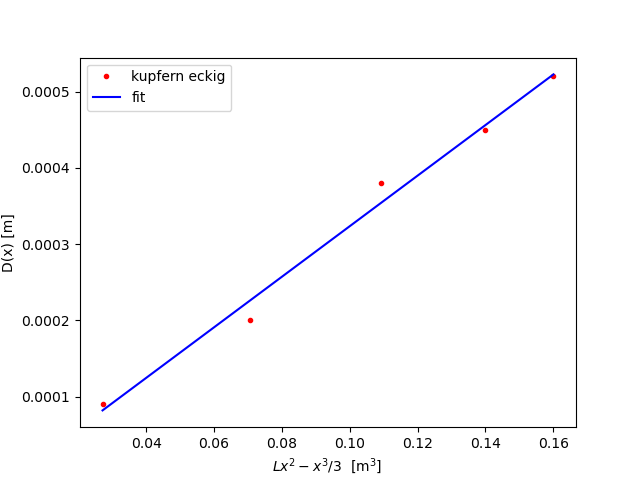
\includegraphics{keb.png}
    \captionof{figure}{Biegung eines kupfernen, eckigen Stabes mit zugehöriger Ausgleichsrechnung, bei beidseitiger Einspannung links vom Aufhängungspunkt.}
\end{figure}

\begin{figure}[H]
    \centering
    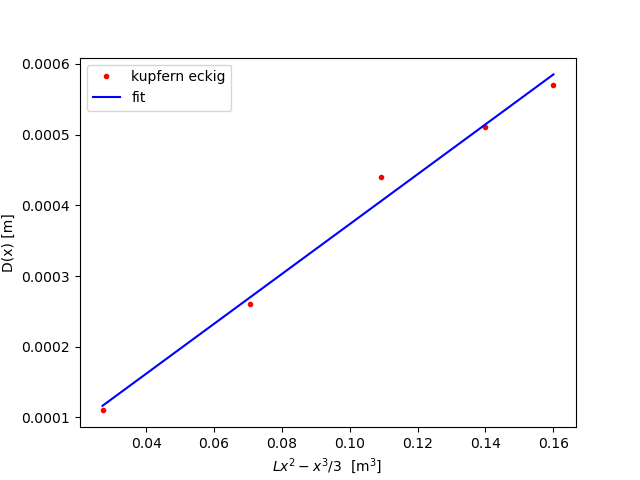
\includegraphics{keb2.png}
    \captionof{figure}{Biegung eines kupfernen, eckigen Stabes mit zugehöriger Ausgleichsrechnung, bei beidseitiger Einspannung rechts vom Aufhängungspunkt.}
\end{figure}

\begin{figure}[H]
    \centering
    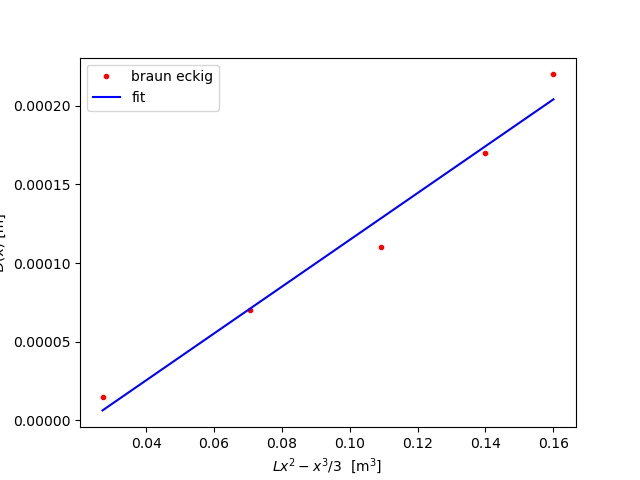
\includegraphics{beb.png}
    \captionof{figure}{Biegung eines braunen, eckigen Stabes mit zugehöriger Ausgleichsrechnung, bei beidseitiger Einspannung links vom Aufhängungspunkt.}
\end{figure}

\begin{figure}[H]
    \centering
    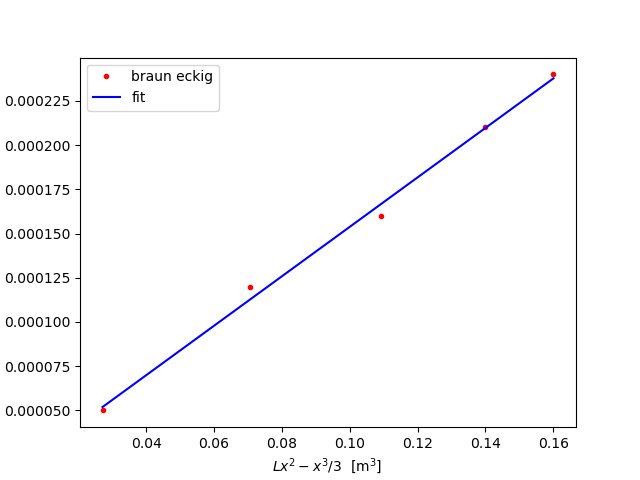
\includegraphics{beb2.png}
    \captionof{figure}{Biegung eines kupfernen, eckigen Stabes mit zugehöriger Ausgleichsrechnung, bei beidseitiger Einspannung rechts vom Aufhängungspunkt.}
\end{figure}

\noindent Die Ausgleichsrechnungen liefern folgende Steigungen:

\begin{align*}
    a_\text{Kupfer, links} &= \SI[separate-uncertainty=true]{3.30(0.21)E-3}{\per \square\metre} \\
    b_\text{Kupfer, links} &= \SI[separate-uncertainty=true]{-0.8(2.3)E-6}{\metre} \\
    a_\text{Kupfer, rechts} &=  \SI[separate-uncertainty=true]{3.50(0.21)E-3}{\per \square\metre} \\
    b_\text{Kupfer, rechts} &= \SI[separate-uncertainty=true]{2.1(2.4)E-5}{\metre} \\
    a_\text{braun, links} &= \SI[separate-uncertainty=true]{1.50(0.14)E-3}{\per \square\metre} \\
    b_\text{braun, links} &= \SI[separate-uncertainty=true]{-3.4(1.6)E-5}{\metre} \\
    a_\text{braun, rechts} &= \SI[separate-uncertainty=true]{1.40(0.06)E-3}{\per \square\metre} \\
    b_\text{braun, rechts} &= \SI[separate-uncertainty=true]{1.4(0.6)E-5}{\metre} \\
\end{align*}

\noindent Mit diesen Steigungen können anschließend die Elastizitätsmodule und deren Fehler (Gleichung \ref{Gauß}) berechnet werden. Dafür wird die folgende Gleichung benötigt:

\begin{displaymath}
    E = \frac{m\, g}{48\, I\, a}
\end{displaymath}

\noindent Die angehängte Masse beträgt hier bei allen Gewichten 2.3408kg. Das Flächenträgheitsmoment ist das gleich wie bei vorherigen Rechnungen mit den eckigen Stäben. Dabei entstehen folgende Werte für die Elastizitätsmodule:

\begin{align*}
    E_\text{Kupfer, links} &= \SI[separate-uncertainty=true]{380(40)}{\giga\pascal} \\
    E_\text{Kupfer, rechts} &= \SI[separate-uncertainty=true]{410(18)}{\giga\pascal}\\
    E_\text{braun, links} &=  \SI[separate-uncertainty=true]{174(11)}{\giga\pascal}  \\
    E_\text{braun, rechts} &= \SI[separate-uncertainty=true]{164(10)}{\giga\pascal} \\
\end{align*}

\subsection{runde Stäbe, beidseitige Einspannung}

Zur Bestimmung dieser Elastizitätsmodule ist das Vorgehen sehr ähnlich dem Vorherigen. Die Werte für die Diagramme stammen allerdings aus den Tabellen \ref{tab:3} und \ref{tab:4}. Die Diagramme sehen diesmal folgendermaßen aus:

\begin{figure}[H]
    \centering
    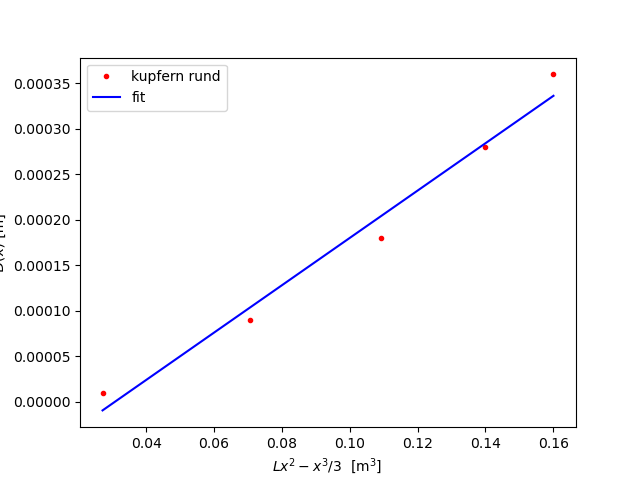
\includegraphics{krb.png}
    \captionof{figure}{Biegung eines kupfernen, runden Stabes mit zugehöriger Ausgleichsrechnung, bei beidseitiger Einspannung links vom Aufhängungspunkt.}
\end{figure}

\begin{figure}[H]
    \centering
    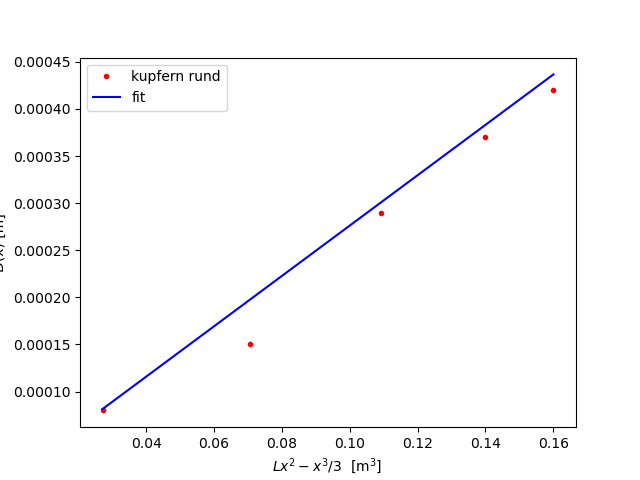
\includegraphics{krb2.png}
    \captionof{figure}{Biegung eines kupfernen, runden Stabes mit zugehöriger Ausgleichsrechnung, bei beidseitiger Einspannung rechts vom Aufhängungspunkt.}
\end{figure}

\begin{figure}[H]
    \centering
    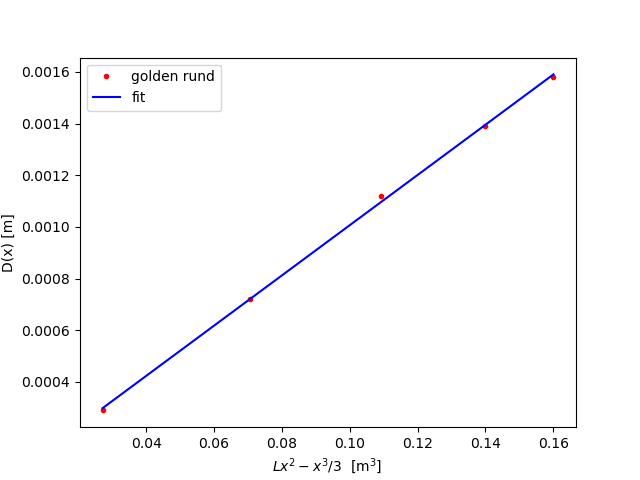
\includegraphics{grb.png}
    \captionof{figure}{Biegung eines goldenen, runden Stabes mit zugehöriger Ausgleichsrechnung, bei beidseitiger Einspannung links vom Aufhängungspunkt.}
\end{figure}

\begin{figure}[H]
    \centering
    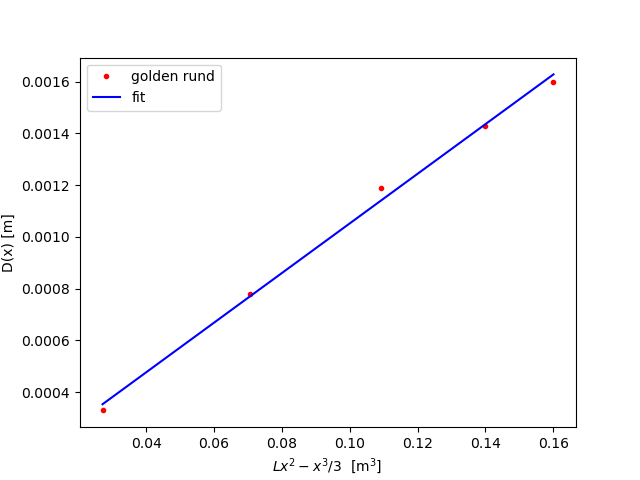
\includegraphics{grb2.png}
    \captionof{figure}{Biegung eines goldenen, runden Stabes mit zugehöriger Ausgleichsrechnung, bei beidseitiger Einspannung rechts vom Aufhängungspunkt.}
\end{figure}

\noindent Die Ausgleichsrechnungen liefern folgende Steigungen:

\begin{align*}
    a_\text{kupfer, links} &= \SI[separate-uncertainty=true]{2.60(0.22)E-3}{\per \square\metre}\\
    b_\text{kupfer, links} &= \SI[separate-uncertainty=true]{8.0(2.5)E-5}{\metre}\\
    a_\text{kupfer, rechts} &= \SI[separate-uncertainty=true]{2.70(0.19)E-3}{\per \square\metre}\\
    b_\text{kupfer, rechts} &= \SI[separate-uncertainty=true]{-0.9(2.1)E-5}{\metre}\\
    a_\text{golden, links} &= \SI[separate-uncertainty=true]{9.70(0.15)E-3}{\per \square\metre}\\
    b_\text{golden, links} &= \SI[separate-uncertainty=true]{3.5(1.7)E-5}{\metre}\\
    a_\text{golden, rechts} &= \SI[separate-uncertainty=true]{9.60(0.34)E-3}{\per \square\metre} \\
    b_\text{golden, rechts} &= \SI[separate-uncertainty=true]{9.4(3.8)E-5}{\metre}\\
\end{align*}

\noindent Mit diesen Steigungen können anschließend die Elastizitätsmodule und deren Fehler (Gleichung \ref{Gauß}) berechnet werden. Dafür wird die folgende Gleichung benötigt:

\begin{displaymath}
    E = \frac{m\, g}{48\, I\, a}
\end{displaymath}

\noindent Die am kupferfarbenen Stab angehängte Masse beträgt 1,7294kg. Die am goldenen Stab angehängte Masse beträgt 2.3408kg. Das Flächenträgheitsmoment ist das gleiche wie bei der vorherigen Rechnung mit runden Stäben. Bei der Rechnung ergeben sich diese Elastizitätsmodule: 

\begin{align*}
    E_\text{kupfer, links} &=  \SI[separate-uncertainty=true]{277(23)}{\giga\pascal}   \\
    E_\text{kupfer, rechts} &= \SI[separate-uncertainty=true]{267(19)}{\giga\pascal}   \\
    E_\text{golden, links} &=  \SI[separate-uncertainty=true]{100.5(1.6)}{\giga\pascal}\\
    E_\text{golden, rechts} &= \SI[separate-uncertainty=true]{102(4)}{\giga\pascal}    \\
\end{align*}

\subsection{Materialbestimmung durch Dichte}

\subsubsection{brauner, eckiger Stab}

Das Gewicht dieses Stabes beträgt 0.4546kg. Er hat einen quadratischen Querschnitt mit Kantenlänge a=1cm. Dazu ist der Stab 59.4cm lang. Daraus ergibt sich eine Dichte von 7653.20$\frac{kg}{m^3}$.
Der Farbe und der dichte nach zu urteilen handelt es sich bei dem Material dieses Stabes um Stahl.

\subsubsection{kupferner, eckiger Stab}

Das Gewicht dieses Stabes beträgt 0.5359kg. Er hat einen quadratischen Querschnitt mit Kantenlänge a=1cm. Dazu ist der Stab 60.2cm lang. Daraus ergibt sich eine Dichte von 8902.00$\frac{kg}{m^3}$.
Der Farbe und der dichte nach zu urteilen handelt es sich bei dem Material dieses Stabes um Kupfer.

\subsubsection{kupferner, runder Stab}

Das Gewicht dieses Stabes beträgt 0.4168kg. Er hat einen runden Querschnitt mit Durchmesser r=1cm. Dazu ist der Stab 60.2cm lang. Daraus ergibt sich eine Dichte von 8811.84$\frac{kg}{m^3}$.
Der Farbe und der dichte nach zu urteilen handelt es sich bei dem Material dieses Stabes um Kupfer.

\subsubsection{goldener, runder Stab}

Das Gewicht dieses Stabes beträgt 0.394kg. Er hat einen runden Querschnitt mit Durchmesser r=1cm. Dazu ist der Stab 60.2cm lang. Daraus ergibt sich eine Dichte von 8329.81$\frac{kg}{m^3}$.
Der Farbe und der dichte nach zu urteilen handelt es sich bei dem Material dieses Stabes um Messing.

\section{Diskussion}

Zu Beginn der Diskussion sind hier nocheinmal alle Elastizitätsmodule gebündelt aufgeführt:

\begin{align*}
    \text{einseitige Einspannung}\\
    E_\text{Stahl, eckig} &=  \SI[separate-uncertainty=true]{223(9)}{\giga\pascal} \\
    E_\text{Kupfer, eckig} &= \SI[separate-uncertainty=true]{122(4)}{\giga\pascal} \\
    E_\text{Kupfer, rund} &= \SI[separate-uncertainty=true]{146.5(2.6)}{\giga\pascal} \\
    E_\text{Messing, rund} &=\SI[separate-uncertainty=true]{89(17)}{\giga\pascal}  \\
    \text{beidseitige Einspannung} \\
    E_\text{Stahl, eckig, links} &=  \SI[separate-uncertainty=true]{380(40)}{\giga\pascal}  \\
    E_\text{Stahl, eckig, rechts} &=  \SI[separate-uncertainty=true]{410(18)}{\giga\pascal}\\
    E_\text{Kupfer, eckig, links} &= \SI[separate-uncertainty=true]{174(11)}{\giga\pascal} \\
    E_\text{Kupfer, eckig, rechts} &=\SI[separate-uncertainty=true]{164(10)}{\giga\pascal} \\
    E_\text{Kupfer, rund, links} &=  \SI[separate-uncertainty=true]{277(23)}{\giga\pascal}   \\
    E_\text{Kupfer, rund, rechts} &= \SI[separate-uncertainty=true]{267(19)}{\giga\pascal}   \\
    E_\text{Messing, rund, links} &= \SI[separate-uncertainty=true]{100.5(1.6)}{\giga\pascal}\\
    E_\text{Messing, rund, rechts} &=\SI[separate-uncertainty=true]{102(4)}{\giga\pascal}    \\
\end{align*}

\noindent Die Literaturwerte der Elastizitätsmodule sind: 

\begin{align*}
    E_\text{Stahl} &= \SI{210}{\giga\pascal} \\
    E_\text{Kupfer} &= \SIrange[range-units=brackets, range-phrase=-]{100}{130}{\giga\pascal} \\
    E_\text{Messing} &= \SIrange[range-units=brackets, range-phrase=-]{78}{123}{\giga\pascal} \\
\end{align*}

\noindent Diese sind aus \cite{E-Modul}.

\noindent Um zu prüfen wie nah die berechneten Werte an den Literaturwerten liegen wird die prozentuale Abweichung 

\begin{equation*}
    \Delta \% = \left\lvert\frac{E_\text{lit}-E_\text{berechnet}}{E_\text{lit}}\right\rvert \cdot 100\%
\end{equation*}

\noindent bestimmt. Dieser Wert lässt dann Aussagen über Güte der berechneten Werte zu und macht die einzelnen Messungen auch noch vergleichbar.

\noindent Auffällig ist hierbei sofort, dass bei der Messung mit der beidseitigen Einspannung des Kupfer Stabes ein systematischer Fehler vorliegen muss. Die Abweichung der Werte, die für das Elastizitätsmodul dabei entstanden weichen deutlich stärker ab als jeder andere Wert. Die Abweichung dieses Wertes beträgt 95.23\%. Bei den anderen Werten ist mit bloßem Auge zu erkennen, dass die Abweichung deutlich geringer ist. Genauer sind hier alle Abweichungen der Werte einmal aufgelistet:

\begin{align*}
    \text{einseitige Einspannung}\\
    \Delta E_\text{Stahl, eckig} &= 6.19\% \\
    \Delta E_\text{Kupfer, eckig} &=  \\
    \Delta E_\text{Kupfer, rund} &= 12.31\% \\
    \Delta E_\text{Messing, rund} &=  \\
    \text{beidseitige Einspannung} \\
    \Delta E_\text{Stahl, eckig, links} &= 80.95\% \\
    \Delta E_\text{Stahl, eckig, rechts} &= 95.23\%\\
    \Delta E_\text{Kupfer, eckig, links} &= 33.85\%\\
    \Delta E_\text{Kupfer, eckig, rechts} &= 26.15\%\\
    \Delta E_\text{Kupfer ,rund, links} &= 113.08\%\\
    \Delta E_\text{Kupfer , rund, rechts} &= 105.38\%\\
    \Delta E_\text{Messing, rund, links} &= \\
    \Delta E_\text{Messing, rund, rechts} &= \\
\end{align*}

\noindent Zu diesen Werten ist zu sagen, dass die Abweichungen, die nicht berechnet wurden nicht 0\% sind. Die Abweichungen wurden nur nicht bestimmt, da das E-modul von Kupfer und Messing in Bereichen angegeben ist. Wenn keine Abweichung bestimmt wurde liegt der berechnete Wert in diesem Bereich. Wenn die Abweichung bestimmt wurde dann immer zu der näheren Grenze des Bereichs. 

\noindent Im Allgemeinen fällt auf, dass die Messung bei einseitiger Einspannung sehr viel genauer funktioniert als die Messung bei beidseitiger Einspannung. Dies könnte zum einen daran liegen, dass die Auslenkungen bei einseitiger Einspannung größer sind. Wenn die Messwerte größer sind haben absolute systematische Fehler wie Ableseungenauigkeiten oder eine schlechtere Eichung der Messuhren einen geringeren prozentualen Einfluss. 

\noindent Außerdem können bei der auswertung der Messung mit einseitiger Einspannung alle Messwerte in einem Diagramm aufgetragen werden und müssen nicht auf zwei aufgeteilt werden. Die Ausgleichsrechnungen laufen bei einseitiger Einspannung also mit der doppelten Menge an Messwerten was den Fehler auch noch verkleinert. 

\noindent Des Weiteren heben die Stäbe bei beidseitiger Einspannung auf einer Seite unweigerlich an. Durch den Druch den der Schraubstock an der einen Seite auf den Stab ausübt hebt sich das andere Ende an. Dies verfälscht zusätzlich die Messwerte.

\noindent Für kleinere Fehler sorgt noch, dass die Stäbe durch häufiges Benutzen im Experiment nicht mehr ganz gerade sind. Eine leichte Vorkrümmung sorgt hier auch noch für kleinere Abweichungen.

\section{Messwerte}

\begin{minipage}{\linewidth}
    \begin{table}[H]
        \centering
    \captionof{table}{brauner, eckiger Stab}
    \begin{tabular}{lll}
        \toprule
        x [cm] & D(x) (einseitig) [mm] & D(x) (beidseitig) [mm] \\
        \midrule
        3  & 0.03 & 0.015 \\
        8  & 0.14 & 0.07  \\
        13 & 0.32 & 0.11  \\
        18 & 0.59 & 0.17  \\
        23 & 0.85 & 0.22  \\
        32 & 1.46 & 0.24  \\
        37 & 1.72 & 0.21  \\
        42 & 1.88 & 0.16  \\
        47 & 2.30 & 0.12  \\
        52 & 3.00 & 0.05  \\
        \bottomrule   
    \end{tabular}
    
    \label{tab:1}
\end{table}
\end{minipage}


\begin{minipage}{\linewidth}
    \begin{table}[H]
        \centering
    \captionof{table}{kupferner, eckiger Stab}
    \begin{tabular}{lll}
        \toprule
        x [cm] & D(x) (einseitig) [mm] & D(x) (beidseitig) [mm] \\
        \midrule
        3  & 0.04 & 0.09 \\
        8  & 0.21 & 0.20 \\
        13 & 0.49 & 0.38 \\
        18 & 0.93 & 0.45 \\
        23 & 1.29 & 0.52 \\
        32 & 2.28 & 0.57 \\
        37 & 2.62 & 0.51 \\
        42 & 3.45 & 0.44 \\
        47 & 4.35 & 0.26 \\
        52 & 5.36 & 0.11 \\
        \bottomrule   
    \end{tabular}
    
    \label{tab:2}
\end{table}
\end{minipage}

\begin{minipage}{\linewidth}
    \begin{table}[H]
        \centering
    \captionof{table}{kupferner, runder Stab}
    \begin{tabular}{llll}
        \toprule
        x [cm] & D(x) (einseitig) [mm] & x2 [cm] & D(x) (beidseitig) [mm] \\
        \midrule
        3  & 0.01 & 3  & 0.01 \\ 
        8  & 0.07 & 8  & 0.09 \\ 
        13 & 0.17 & 13 & 0.18 \\ 
        18 & 0.32 & 18 & 0.28 \\ 
        23 & 0.48 & 23 & 0.36 \\ 
        28 & 0.67 & 32 & 0.42 \\ 
        33 & 0.82 & 37 & 0.37 \\ 
        38 & 1.02 & 42 & 0.29 \\ 
        43 & 1.32 & 47 & 0.15 \\ 
        48 & 1.49 & 52 & 0.08 \\ 
        \bottomrule   
    \end{tabular}
    
    \label{tab:3}
\end{table}
\end{minipage}

\begin{minipage}{\linewidth}
    \begin{table}[H]
        \centering
    \captionof{table}{goldener, runder Stab}
    \begin{tabular}{llll}
        \toprule
        x [cm] & D(x) (einseitig) [mm] & x2 [cm] & D(x) (beidseitig) [mm] \\
        \midrule
        3  & 0.06 & 3  & 0.29 \\ 
        8  & 0.26 & 8  & 0.72 \\ 
        13 & 0.61 & 13 & 1.12 \\ 
        18 & 1.10 & 18 & 1.39 \\ 
        23 & 1.70 & 23 & 1.58 \\ 
        28 & 2.46 & 32 & 1.60 \\ 
        33 & 3.1  & 37 & 1.43 \\ 
        38 & 3.8  & 42 & 1.19 \\ 
        43 & 4.75 & 47 & 0.78 \\ 
        48 & 5.37 & 52 & 0.33 \\ 
        \bottomrule   
    \end{tabular}
    
    \label{tab:4}
\end{table}
\end{minipage}